\section{GAN}
	
	GAN:我劝PixelCNN和VAE,先把生成的这个理念先搞懂.你VAE什么的都在搞概率论,他能搞吗?搞不了,没这个能力知道吗?
	
	minimax game:
	\begin{equation}
		\min _{\theta_{g}} \max _{\theta_{d}}\left[\mathbb{E}_{x \sim p_{d a t a}} \log D_{\theta_{d}}(x)+\mathbb{E}_{z \sim p(z)} \log \left(1-D_{\theta_{d}}\left(G_{\theta_{g}}(z)\right)\right)\right]
	\end{equation}

	交替训练.防止梯度相似?\marginpar{discriminator: 
		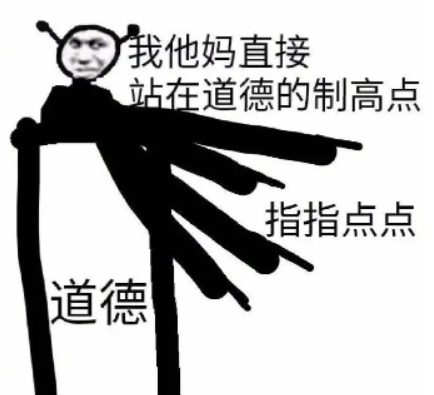
\includegraphics[scale=0.28]{figures/ddgg.png}}
	
	但是有一点值得注意:上式中$\log(1-x)$这一函数在$x$接近$0$时梯度非常小.而训练之初,discriminator可以轻易辨别出generator生成的图片为假,而generator的梯度又太小,于是就形成了discriminator把generator按在墙角使劲打,后者还跑不出去.
	
	
	
	总之,这个loss对于generator是很不利的.
	
	Non-Saturating Loss functions.
	
	如何衡量网络的表现?很难有客观的度量.
	
	Qualitative GAN Generator Evaluation
	
	主观度量.Nearest neighbors: to detect overfitting, generated samples are shown next to their nearest neighbors in the training set.这也是我们之前interpolation要求渐变的原因,防止你只学了个记忆功能.如果是这样,那么连续变化会有非常明显的不连续.
	
	User study
	
	Mode drop and mode collapse: Over datasets with known modes (e.g. a GMM or a labeled dataset), modes are computed as by measuring the distances of generated data to mode centers.
	
	mode collapse:假如对所有z都输出同一张gt呢?我们并没有规定生成所有类型的图片,假如网络只生成了一小部分类型(drop),或者只生成一张图(mode collapse).猫捉老鼠:g总是只生成一张,d总是说这是假的.(mode chasing)根源:VAE要求所有类型都为真,而GAN则只需要保证"我生成的"图片真.这也是GAN发展早期最棘手的问题之一.
	
	Quantitative Measurement: FID
	
	FID实际上就是将gt和生成图片都转换到一个特征空间,随后认为其符合正态,度量其统计参数.
	
	\begin{equation}
		\operatorname{FID}(r, g)=\left\|\mu_{r}-\mu_{g}\right\|_{2}^{2}+\operatorname{Tr}\left(\Sigma_{r}+\Sigma_{g}-2\left(\Sigma_{r} \Sigma_{g}\right)^{\frac{1}{2}}\right)
	\end{equation}
	
	FID measure\marginpar{\kaishu 既关心真不真,也关心全不全.} is sensitive to image distortions. From upper left to lower right: Gaussian noise, Gaussian blur, implanted black rectangles, swirled images, salt and pepper noise, and CelebA dataset contaminated by ImageNet images.
	
	GAN在语义上的加减:生成好的图片的网络,其隐变量也必然学习了一些好的特征.latent space structure也必然很好.
	